\documentclass{beamer}
%\documentclass{abntex}

% Pacotes
\usepackage[T1]{fontenc}
\usepackage[utf8]{inputenc}
\usepackage[portuguese]{babel}


%% Configurações do Template, Imagem de Fundo[../template7.jpg], e Tema de apresentação[Madrid]
\usebackgroundtemplate{
	
\includegraphics[width=\paperwidth,
	height=\paperheight]{../BackGround8.jpg}
}
\usetheme{Madrid}

%% Mudança de dimenções da apresentação
\mode<presentation>


  \title[Introdução]{\Huge{Introdução ao \LaTeX}}

  \author[Branquinho]{Pedro Gomes Branquinho \\
    \text{\scriptsize{pedro.branquinho@usp.br}}}
  \date[Lógica/Estrutura]{\scriptsize{Mini-curso de \LaTeX} \\ Universidade de São Paulo - DEMAR}




  \begin{document}


{\usebackgroundtemplate{
\includegraphics[width=\paperwidth]{../Imagens/TP.jpg}}
\begin{frame}
  \titlepage
\end{frame}
}
%\begin{frame}
%\frametitle{Apresentação em \LaTeX}
%\tableofcontents[pausecontents]
%\end{frame}

\begin{frame}
  \section{Motivações}
  \frametitle{Motivações}

  \begin{enumerate}
  \item<1->{Programação Unificada}
  \item<5->{Flexibilidade Computacional}
  \item<2->{Open Source}
  \item<3->{Estruturas Reutilizáveis -- Bottom-up}
  \item<4->{Fácil Compartilhamento}
  \end{enumerate}


\end{frame}

\begin{frame}

  \section{O que é um Ambiente Unificado?}
  \frametitle{O que é um Ambiente Unificado?}
  \pause
  \begin{Definition}[Definição]
    Um \alert{ambiente unificado} é aquele em que sua memória psicológica, bem como
    física, pode ser (re)utilizada de forma intuitiva. Pois, a estrutura do ambiente é
    homogêneo; o que muda são os temas ambientais.
    \end{Definition}
    \pause

    \begin{example}[Exemplos]
      \begin{itemize}

      \item O Emacs, Vim, Atom, Visual Studio, etc. são interfaces gráficas unificadas. O
        Emacs recebe título de IDE(Integrated Development Environment)

        \pause

      \item Jupiterweb, Moodle, Dedalus são sitemas integrados acadêmicos da
        USP.
        \pause
      \item O HTML + CSS são linguagens marcadoras de texto para produção web.
        \pause
      \item O \alert{\LaTeX} é uma linguagem - marcadora de texto - para produção de documentos
        que tenham conteúdo multimídia.
      \end{itemize}
    \end{example}
\end{frame}


\begin{frame}

  \section{Open Source}
  \pause

  \begin{block}{Questões já resolvidas}
    \begin{itemize}
    \item<3->\alert{Criar} uma Linguagem, ou um Compilador, que recebe informações em formato
      texto, imagem, vídeo etc., e retorna-as editadas, como o
      usuário comanda. (Donald Knuth, criador de \TeX -- 12 prêmios
      internacionais em Matemática e Computação)
    \item<4-> Pacotes para 80\% das formatações utilizadas em teses,
      livros, folhetos, e matemática (Leslie Lamport - Prêmio Turing)
    \item<5->{Modelos de documentos, escritos nessa linguagem, sob as
        normas  ABNT} (UnB - Arquitetura da Informação)
    \item<6->{Modelos de um congresso, ou universidade, em específico}
    \item<6->{Formatação científico-matemática}
    \item<6->{etc}
    \end{itemize}
  \end{block}

  \begin{block}{O que ainda falta?}
    \begin{itemize}
    \item<1-> Tudo aquilo que seria uma mão na roda, \alert{E} não
        existe.
    \end{itemize}
  \end{block}
\end{frame}


\begin{frame}
  \section{Instalação em Linux/Unix}
  \frametitle{Instalação em Linux ou Unix}
  Entrar no site github.com, e pesquisar por LaTeX EEL.

  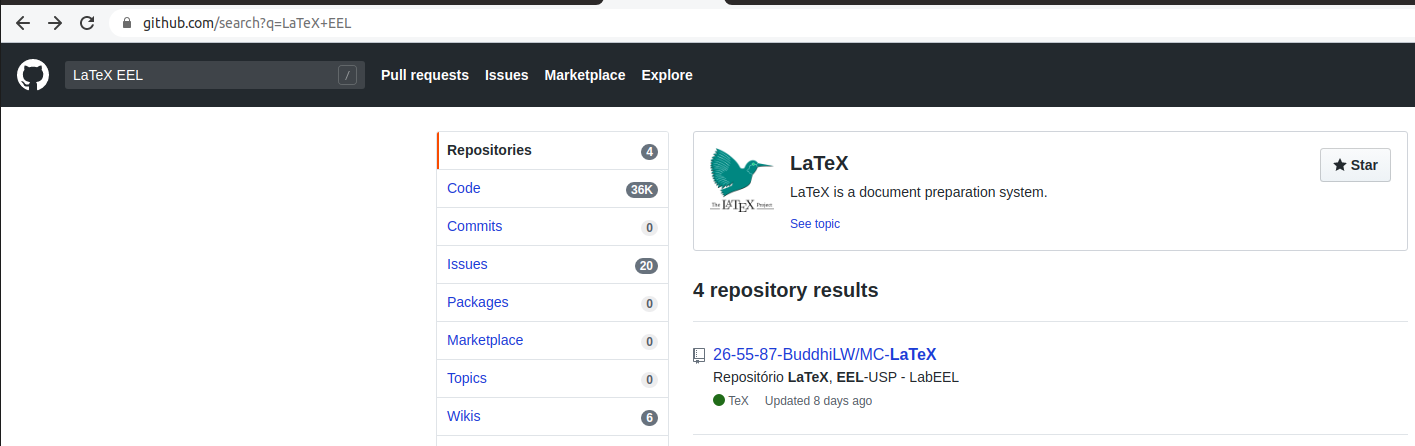
\includegraphics[scale=0.2]{../Imagens/MC1.png}

  \pause

  Baixar, o repositório:

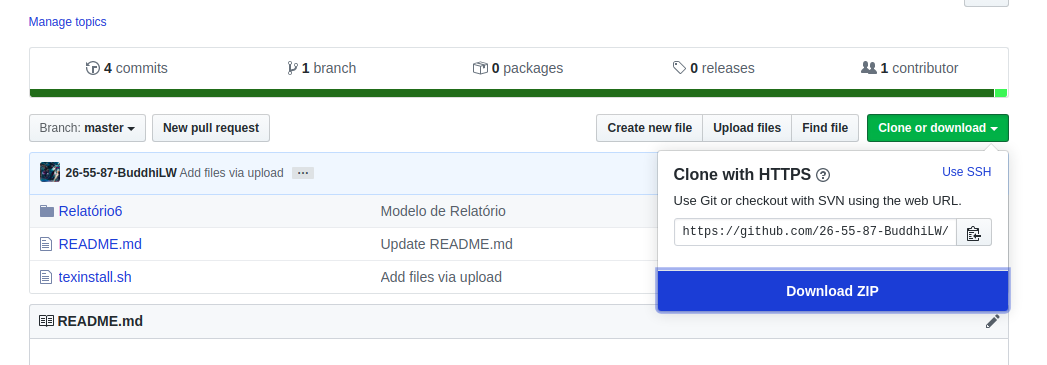
\includegraphics[scale=0.2]{../Imagens/MC3.png}



\end{frame}

\begin{frame}
  \frametitle{Instalação em Linux ou Unix}
  Acessar o diretório com os arquivos baixados, descompactados. E,
  abrir o terminal, no diretório.

  \begin{center}
  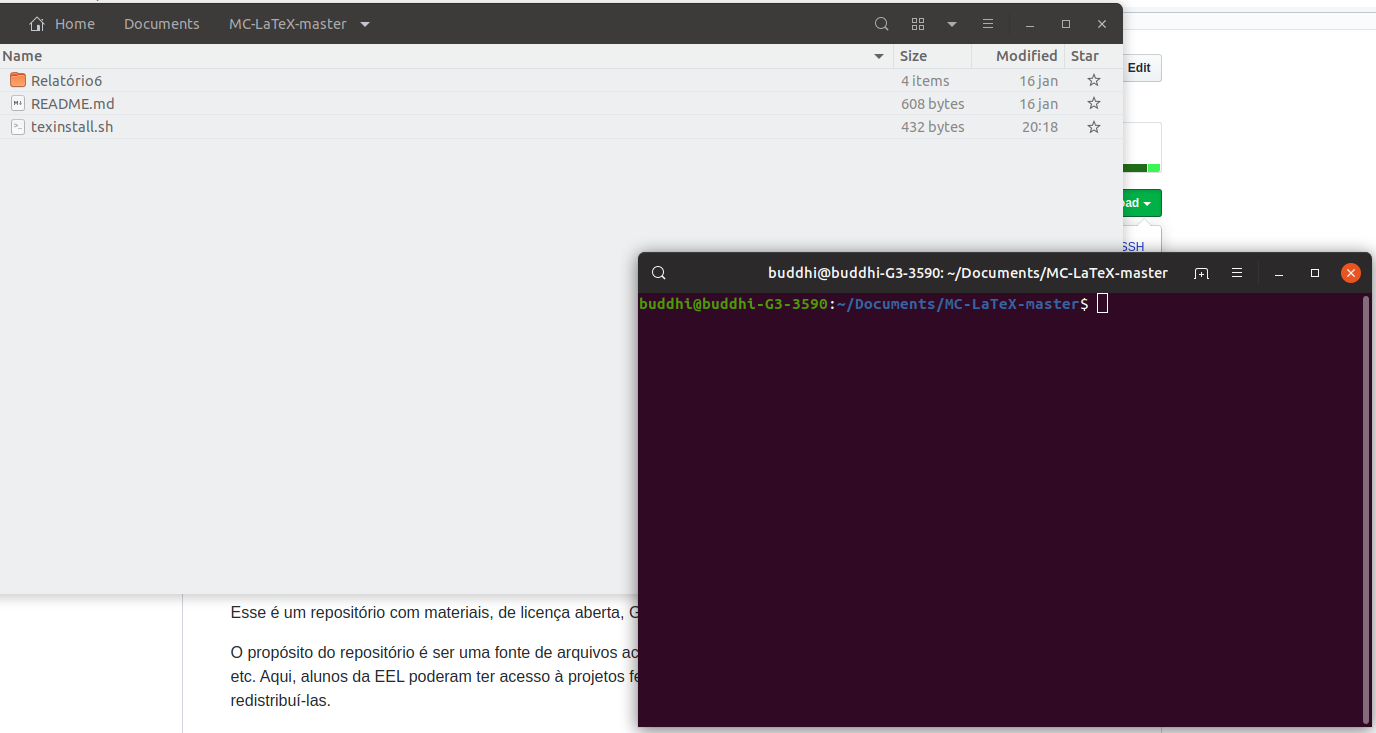
\includegraphics[scale=0.15]{../Imagens/MC4.png}
  \end{center}

  \pause

  Executar o script `'sudo ./texinstall.sh':

  \begin{center}
  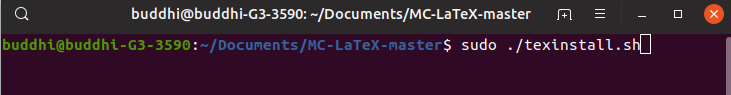
\includegraphics[scale=0.4]{../Imagens/MC5.png}
  \end{center}

\end{frame}


\begin{frame}
  \frametitle{Instalação em Linux ou Unix}

  Ou, após, descompactar o arquivo, comande 'sudo chmod +x [diretório
  arquivo.sh]'. E, por fim, comande '[diretório do arquivo]'

  \begin{center}
    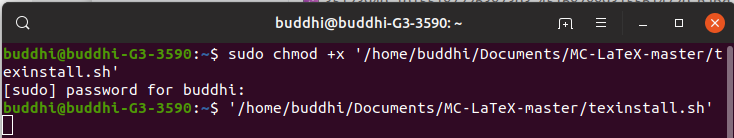
\includegraphics[scale=0.4]{../Imagens/MC6.png}
  \end{center}

  É possível escrever o diretório do arquivo, simplesmente
  arrastando-o ao terminal.

\end{frame}


\begin{frame}

  \section{Instalação em Windows}

  \frametitle{Instalação em Windows, MikTex e TeXstudio}

  Acesse o site 'texstudio.org', clicke na aba à esquerda 'Downloads',
  e instale o arquivo installer.exe. Utilize o instalador.

  \begin{center}
    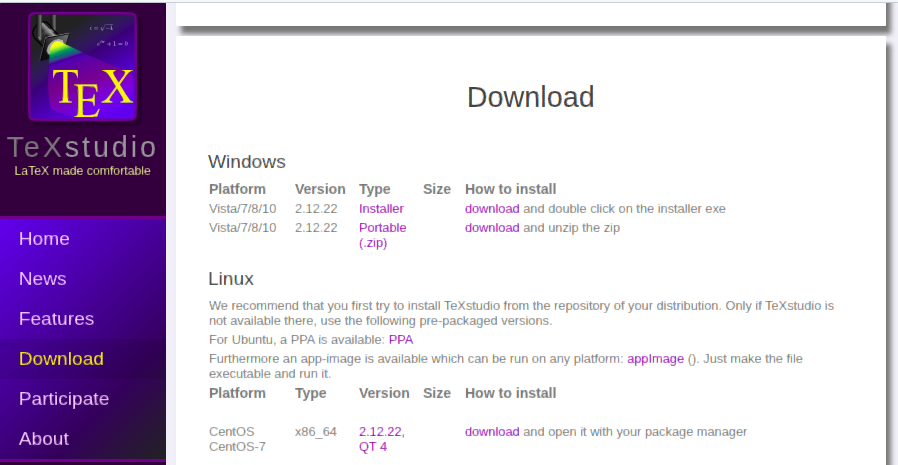
\includegraphics[scale=0.15]{../Imagens/W1.png}
  \end{center}

  \pause

  Acesse o site 'miktex.org/download', instale a opção
  windows. Execute o arquivo .exe, e complete a instalação.

  \begin{center}
    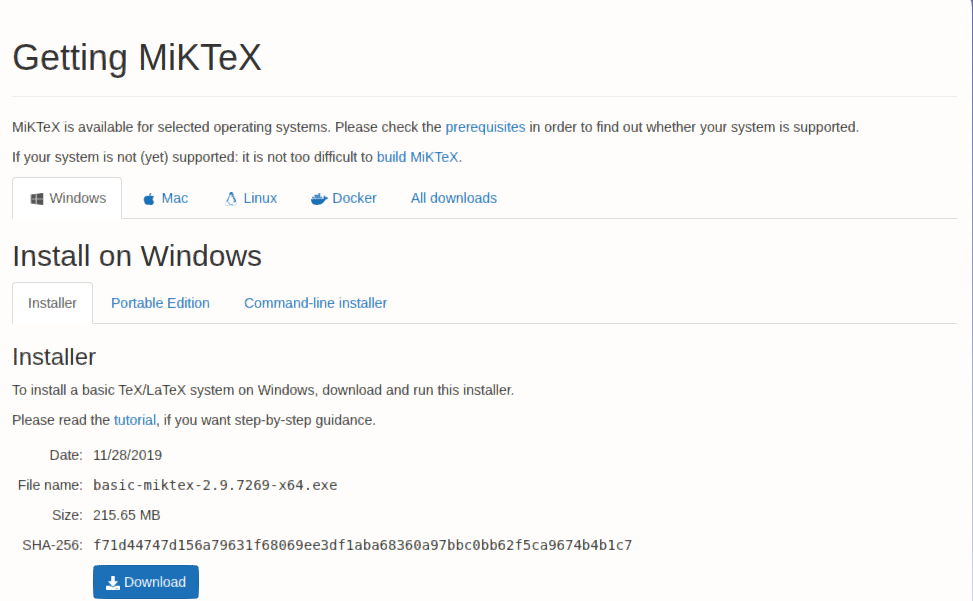
\includegraphics[scale=0.16]{../Imagens/W2.png}
  \end{center}

\end{frame}



\begin{frame}

  \section{TeXstudio, funcionalidades}
  \frametitle{Ambiente de Programação, TeXstudio}
  Acesse no seu computador TeXstudio
  \begin{center}
  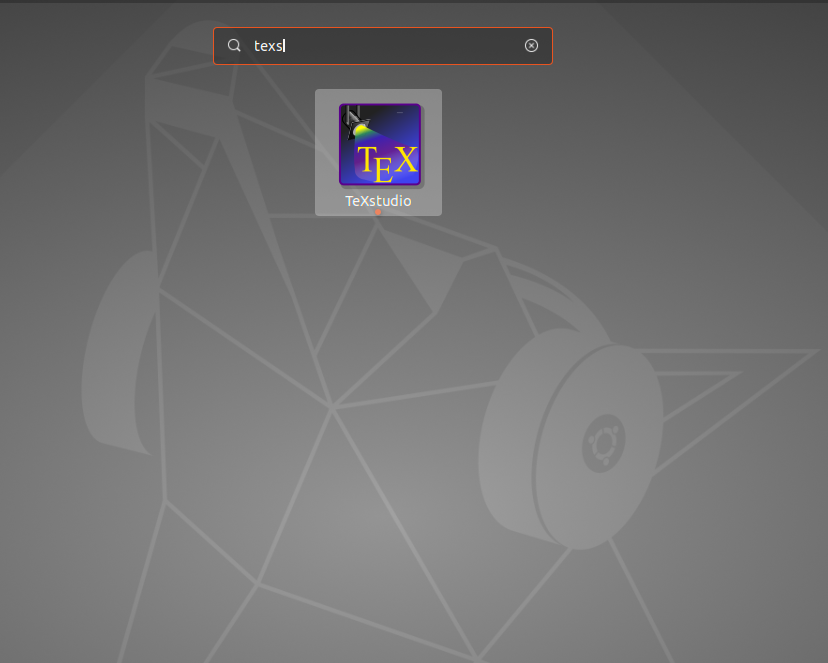
\includegraphics[scale=0.10]{../Imagens/Am1.png}
  \end{center}

  \pause

  \begin{center}
  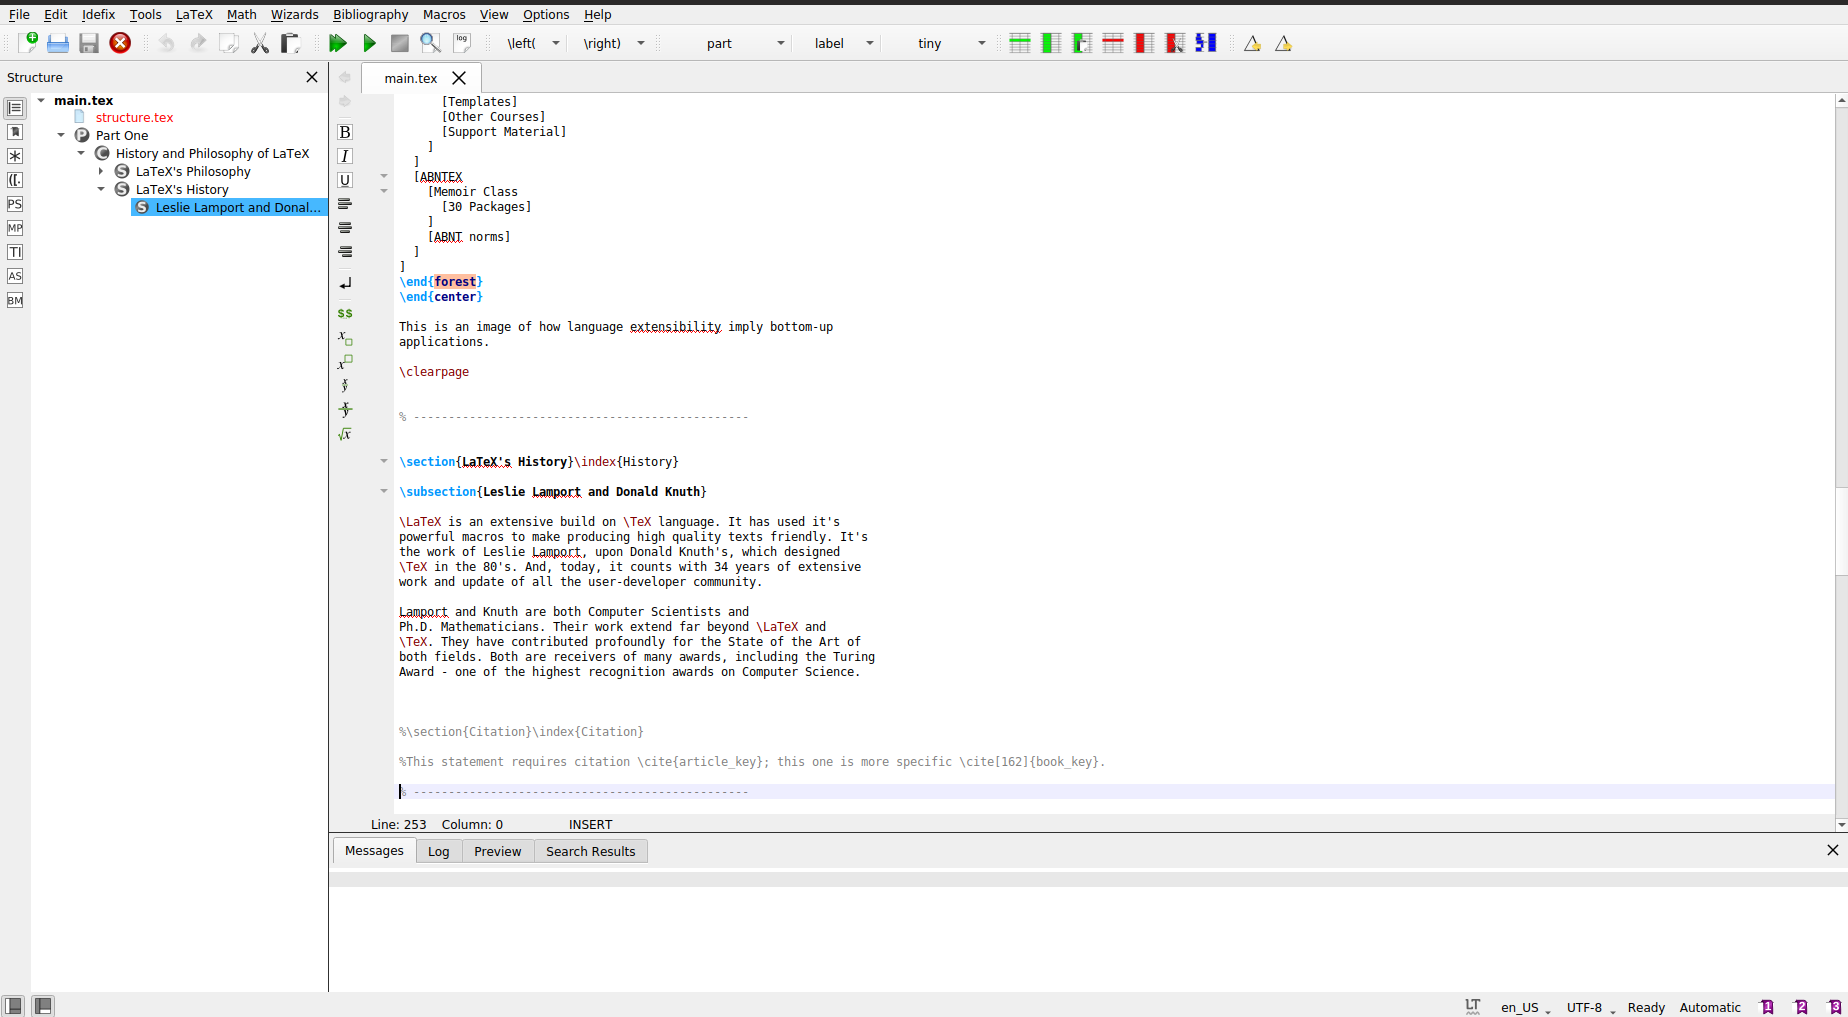
\includegraphics[scale=0.15]{../Imagens/Am2.png}
\end{center}


\end{frame}

\begin{frame}

  \frametitle{Autocomplete}
  Uma das ferramentas mais importante no TeXstudio, e ambientes de
  programação é o 'Autocomplete'.

  \begin{center}
    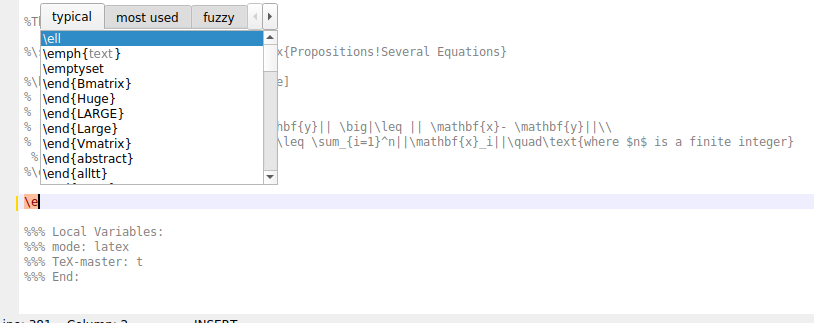
\includegraphics[scale=0.25]{../Imagens/Am3.png}
  \end{center}


  \begin{center}
    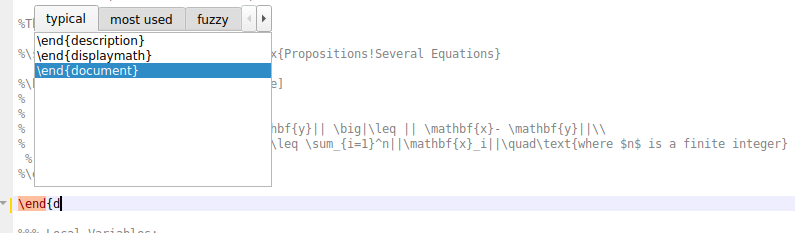
\includegraphics[scale=0.30]{../Imagens/Am4.png}
  \end{center}


\end{frame}



\begin{frame}

  \frametitle{Compilador e Preview}
  É possível Compilar arquivos pressionando 'F6'. E, para ativar o
  Preview, pressionando 'F7'.

  \begin{center}
    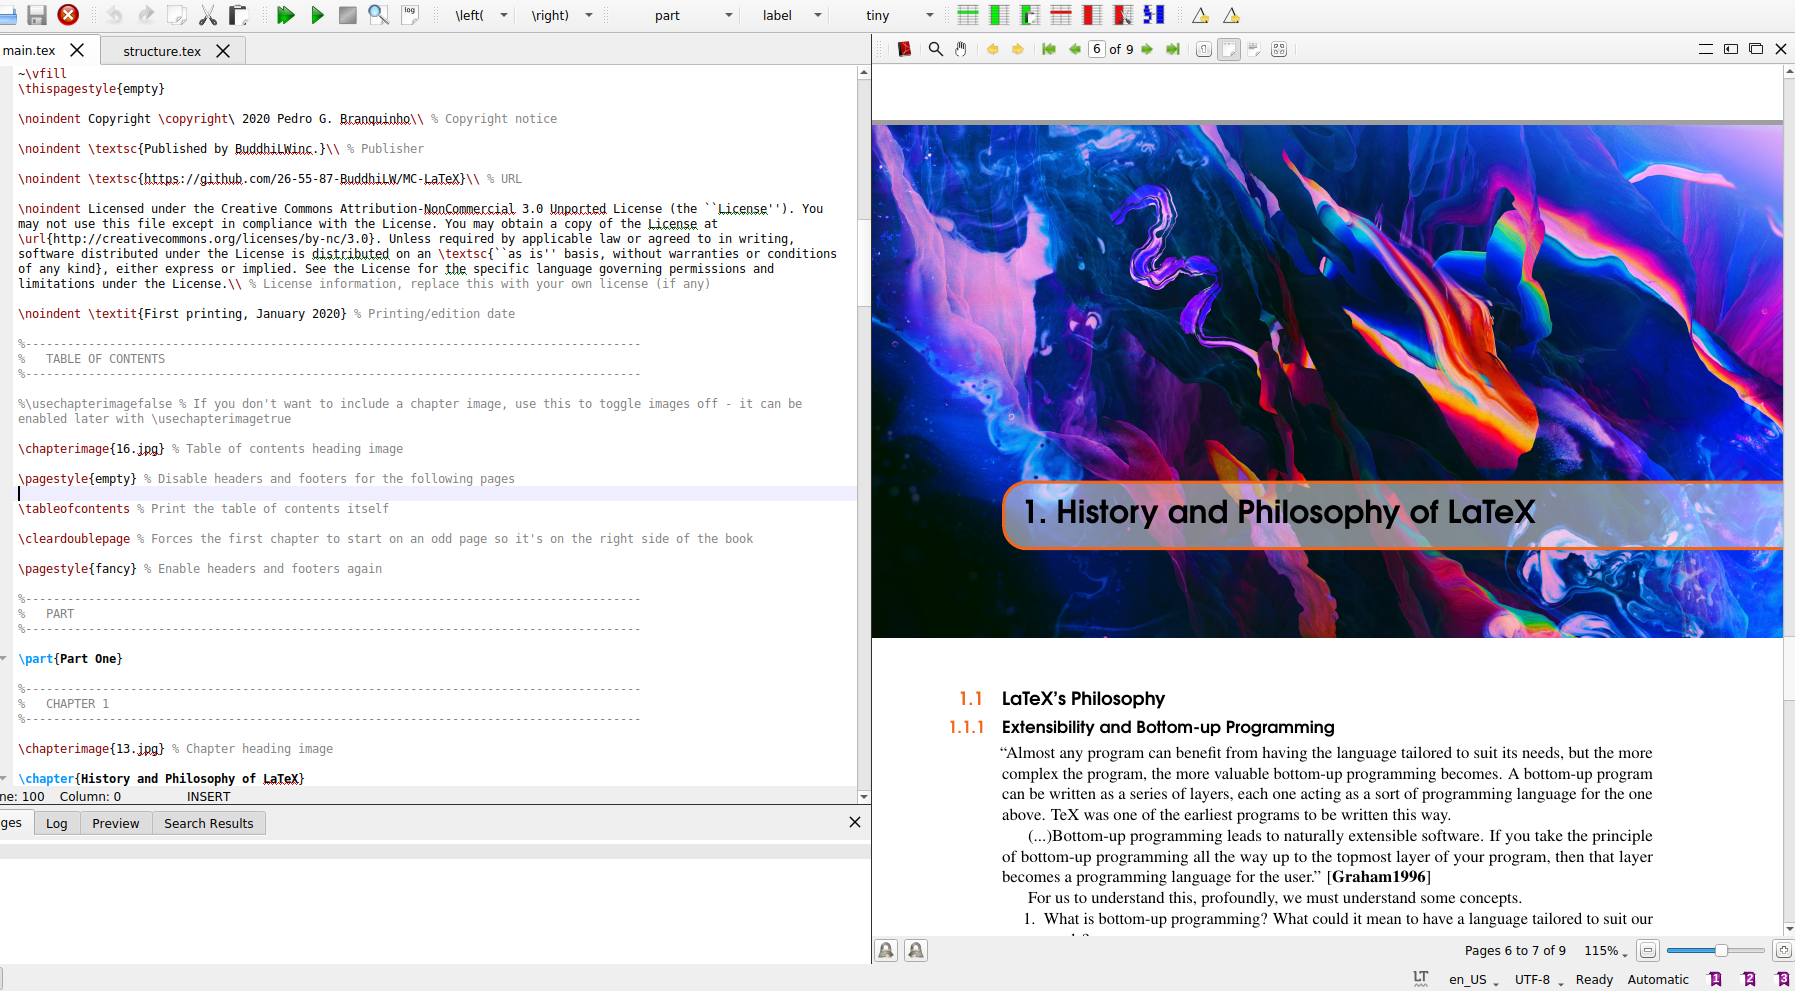
\includegraphics[scale=0.17]{../Imagens/Am6.png}
  \end{center}


\end{frame}


\begin{frame}

  \section{Pacotes, Documentação, e Templates}
  \frametitle{Pacotes e Documentação}
  Um site fundamental, para o aprofundamento do conhecimento de
  pacotes específicos, utilizados em um
  template é o ctan.org. CTAN é a sigla para Comprehensive TEX Archive Network.
  \begin{center}
    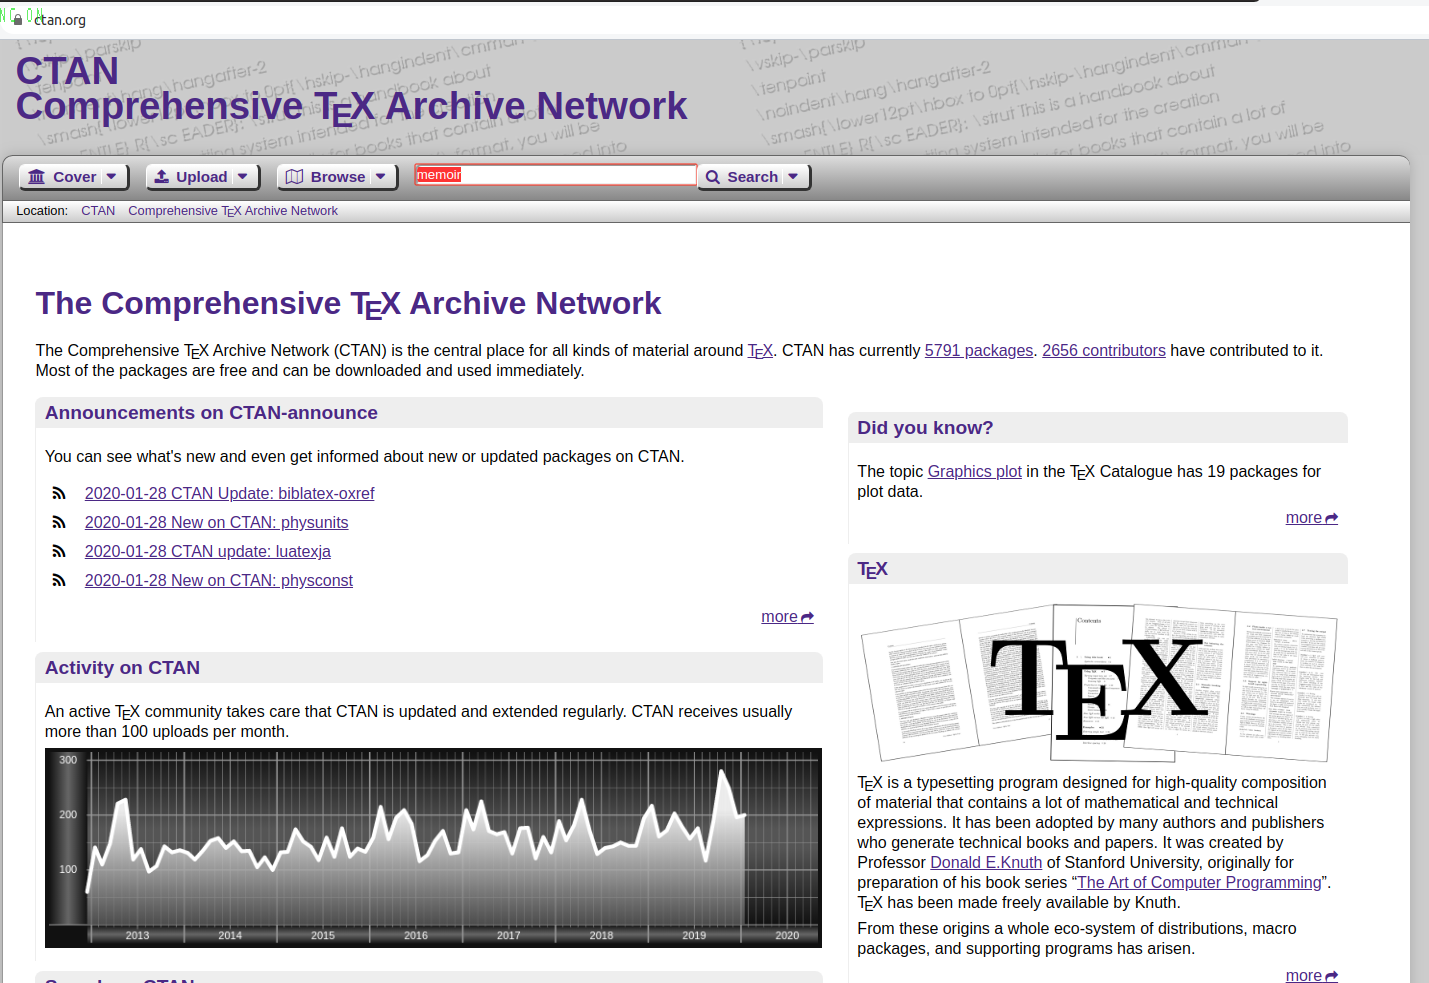
\includegraphics[scale=0.20]{../Imagens/CTAN2.png}
  \end{center}

\end{frame}



\begin{frame}
  \frametitle{Pacotes e Documentação}
  Exemplo: na página da procura ``memoir'', encontramos fontes de
  documentação do pacote. O manual básico nos explica as minúcias do
  funcionamento do pacote. Assim, podemos dominar o funcionamento da formatação
  um documento.
  \begin{center}
    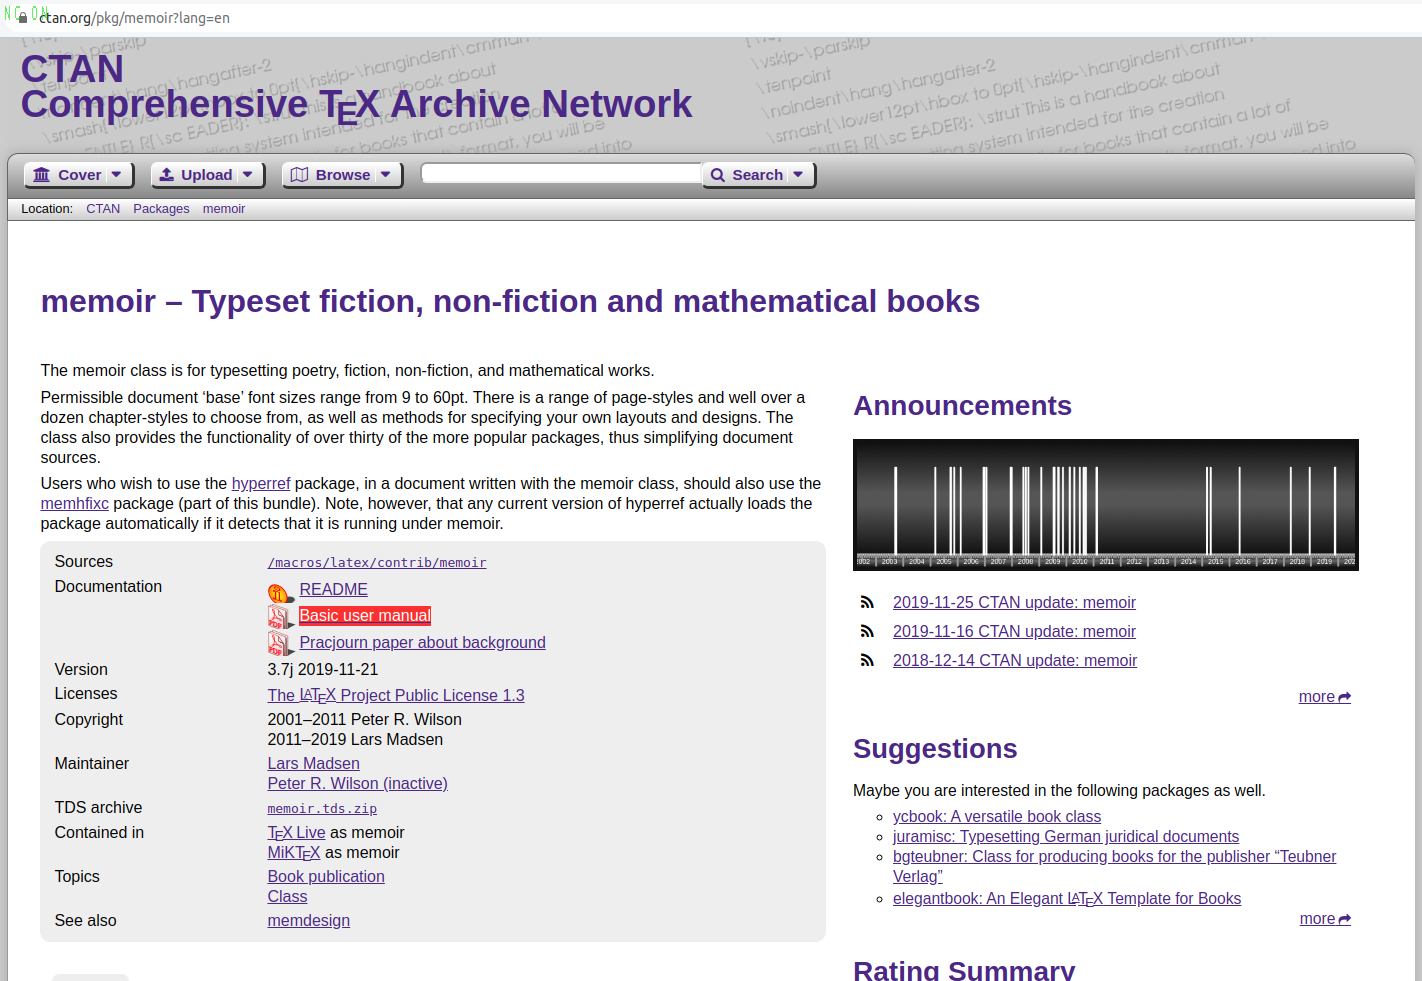
\includegraphics[scale=0.18]{../Imagens/CTAN3.png}
  \end{center}

\end{frame}





\begin{frame}

  \frametitle{Overleaf}
  Na prática, utilizamos templates parcialmente prontos para nossa
  aplicação. Um site-repositório de templates é ``overleaf.com''.

  \begin{center}
  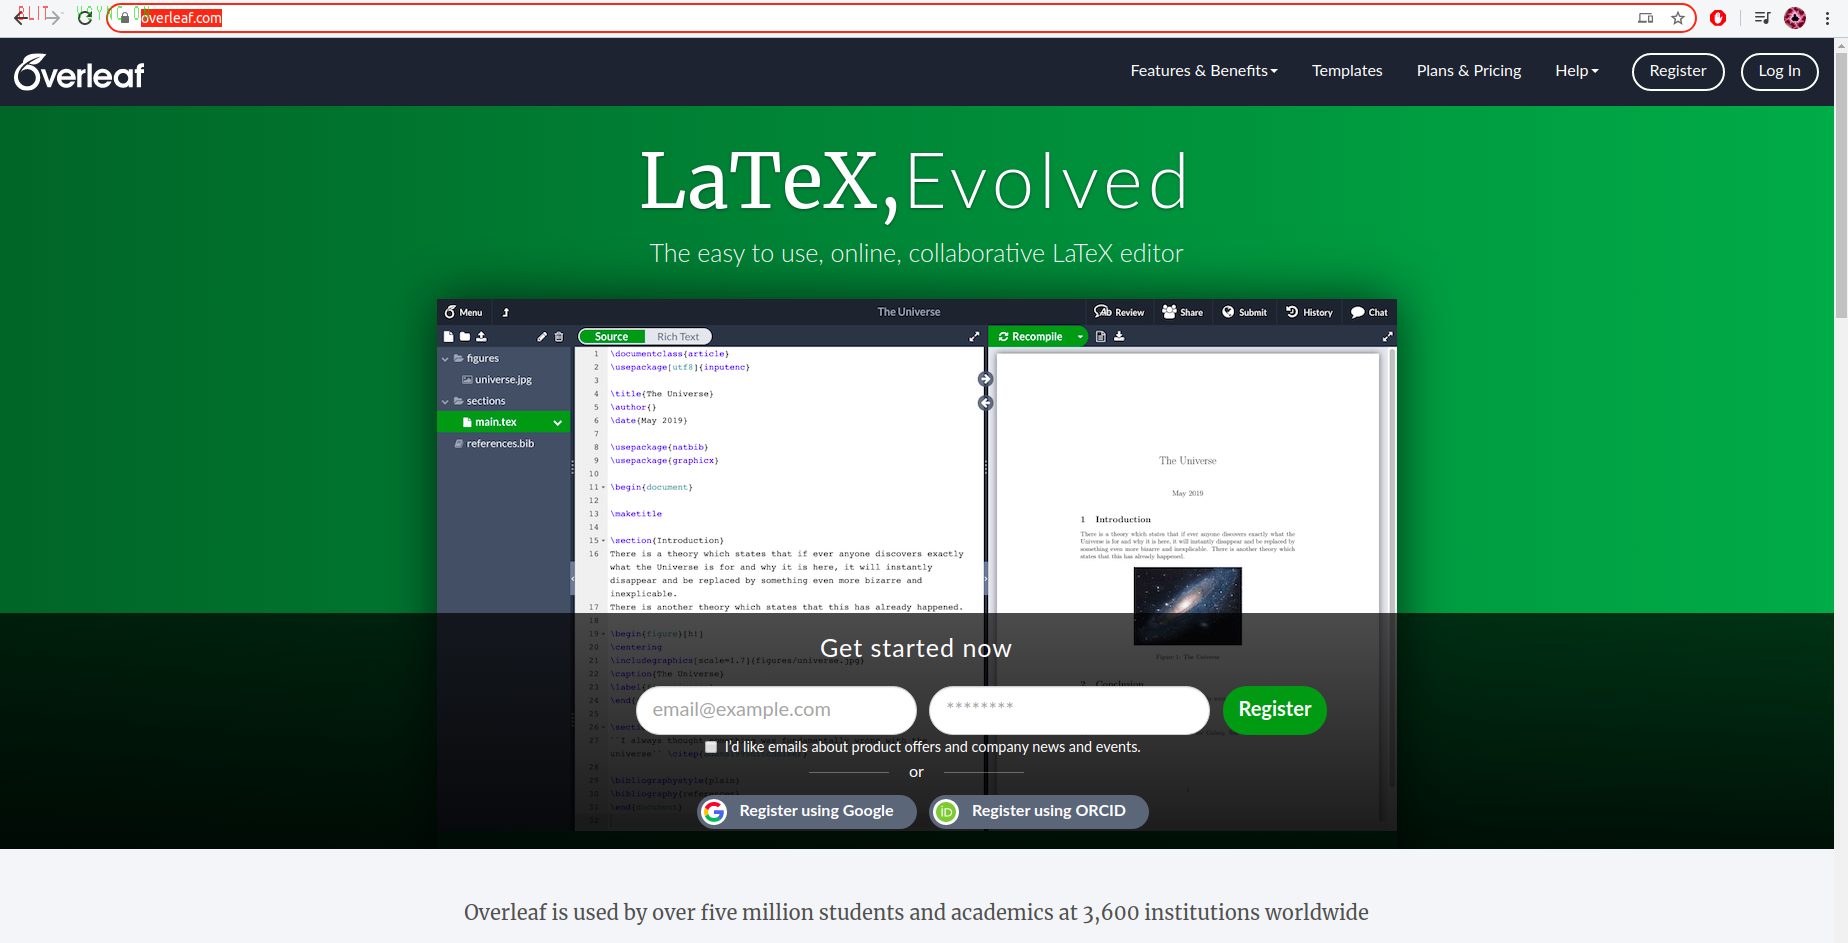
\includegraphics[scale=0.17]{../Imagens/OVERL1.png}
  \end{center}


\end{frame}




\begin{frame}
  \frametitle{Overleaf, Secção Templates}
  Na secção de ``Templates'', encontramos sub-secções de procura,
  particionado pela natureza do trabalho.
  \begin{center}
    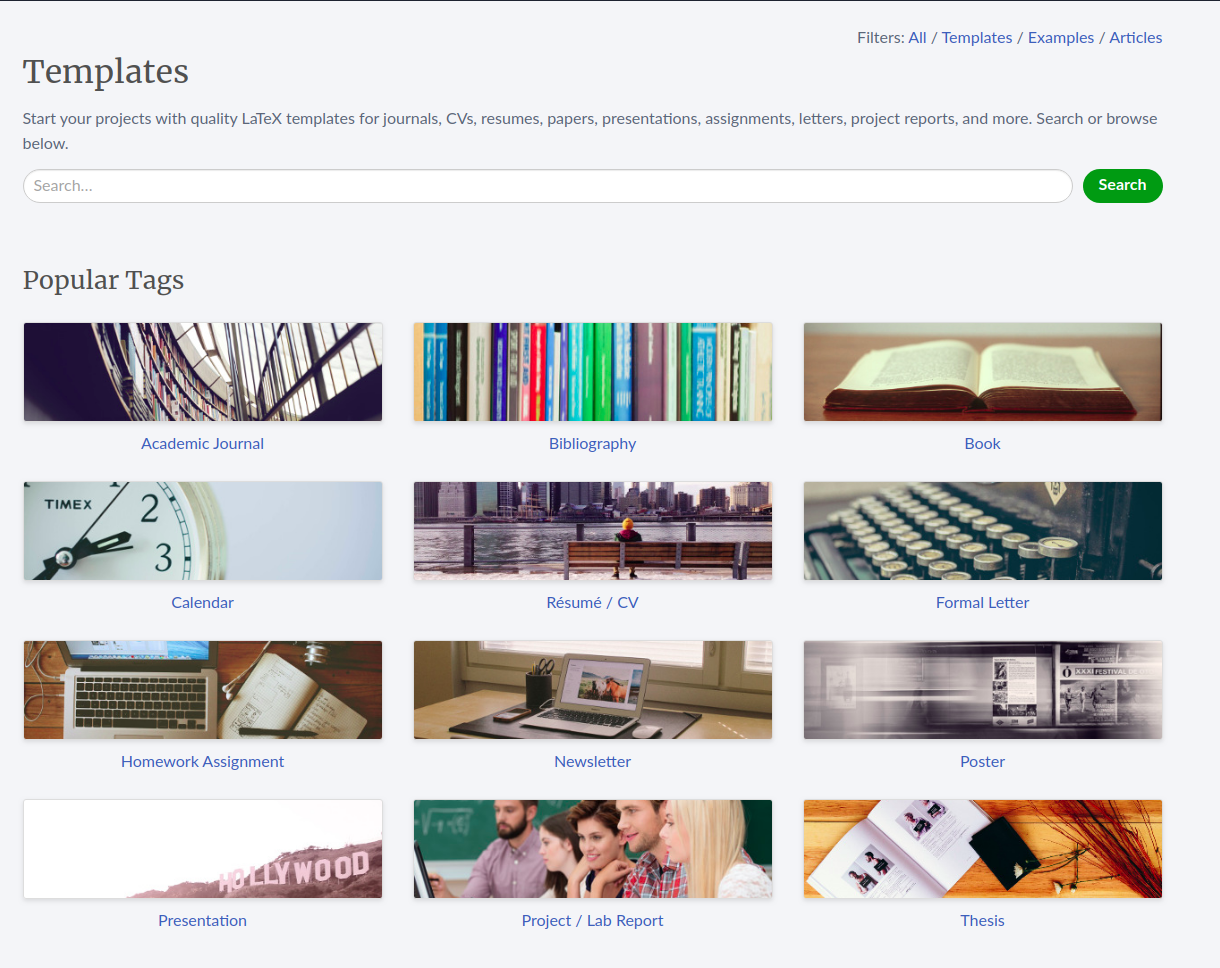
\includegraphics[scale=0.20]{../Imagens/OVERL2.png}
  \end{center}

\end{frame}


\begin{frame}
  \section{Utilização de Template}
  \frametitle{Utilizando Templates da EEL-USP}
  Utilizaremos o arquivo ``Relatório6'', o qual estava dentro do
  conjunto de arquivos baixados, do repositório no GitHub.

  \begin{center}
    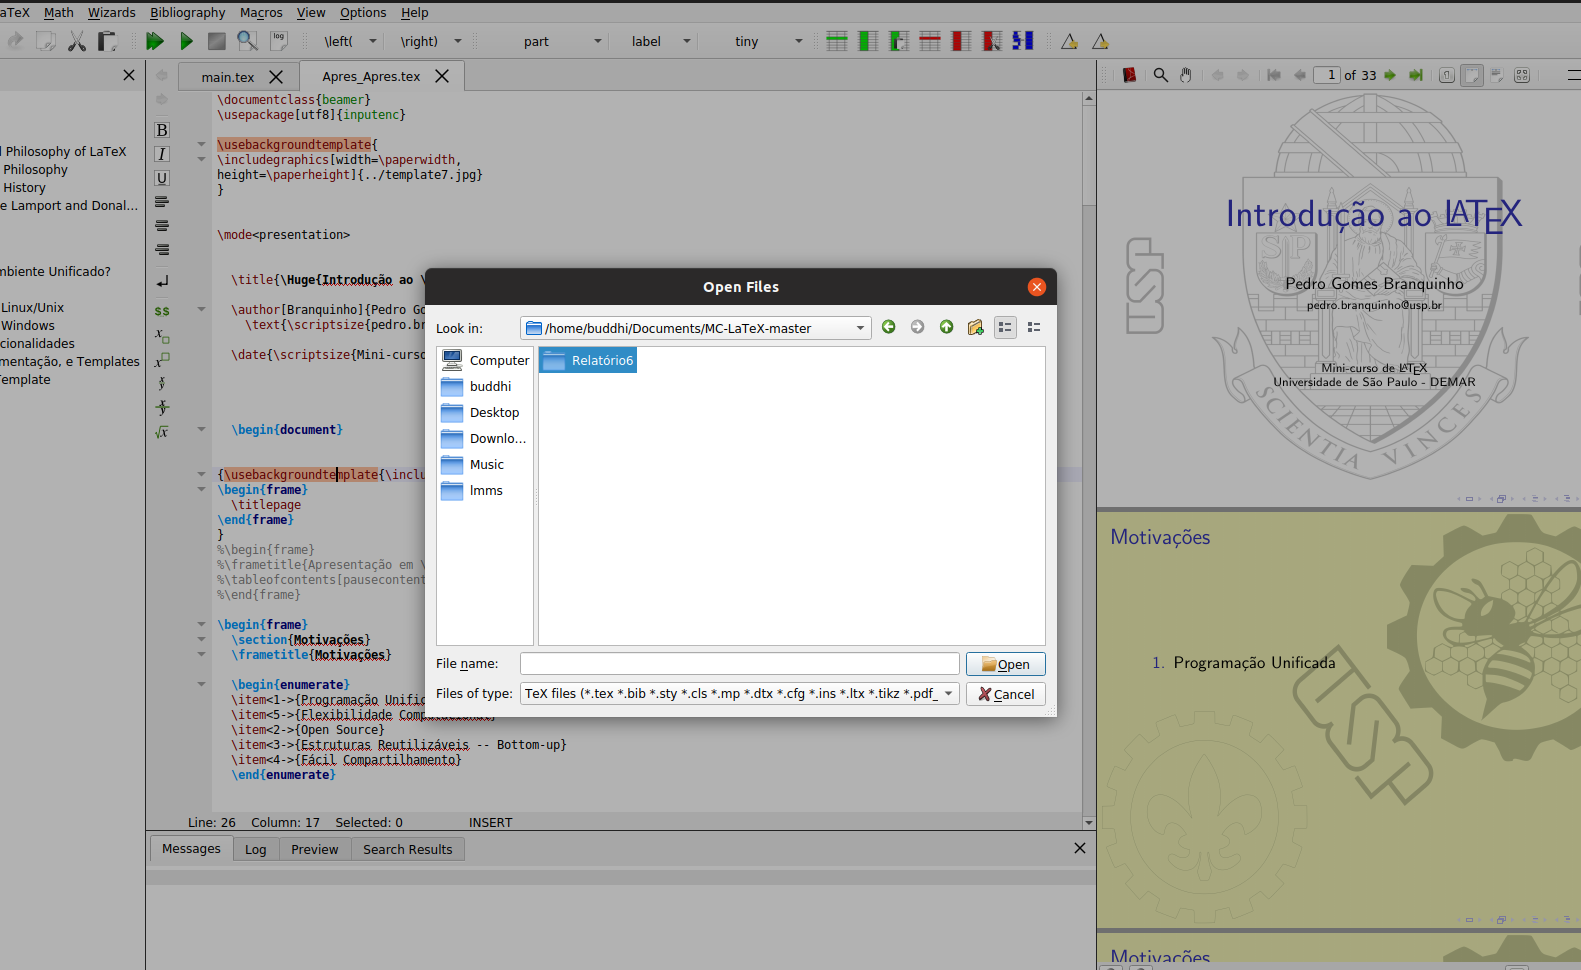
\includegraphics[scale=0.20]{../Imagens/ST1.png}
  \end{center}
\end{frame}



\begin{frame}

  \frametitle{Utilizando Templates da EEL-USP}

Abrindo o arquivo ``Relatório6/Relatório6.tex'' dentro do TeXstudio,
Compile (F6) e Visualize (F7).

\begin{center}
  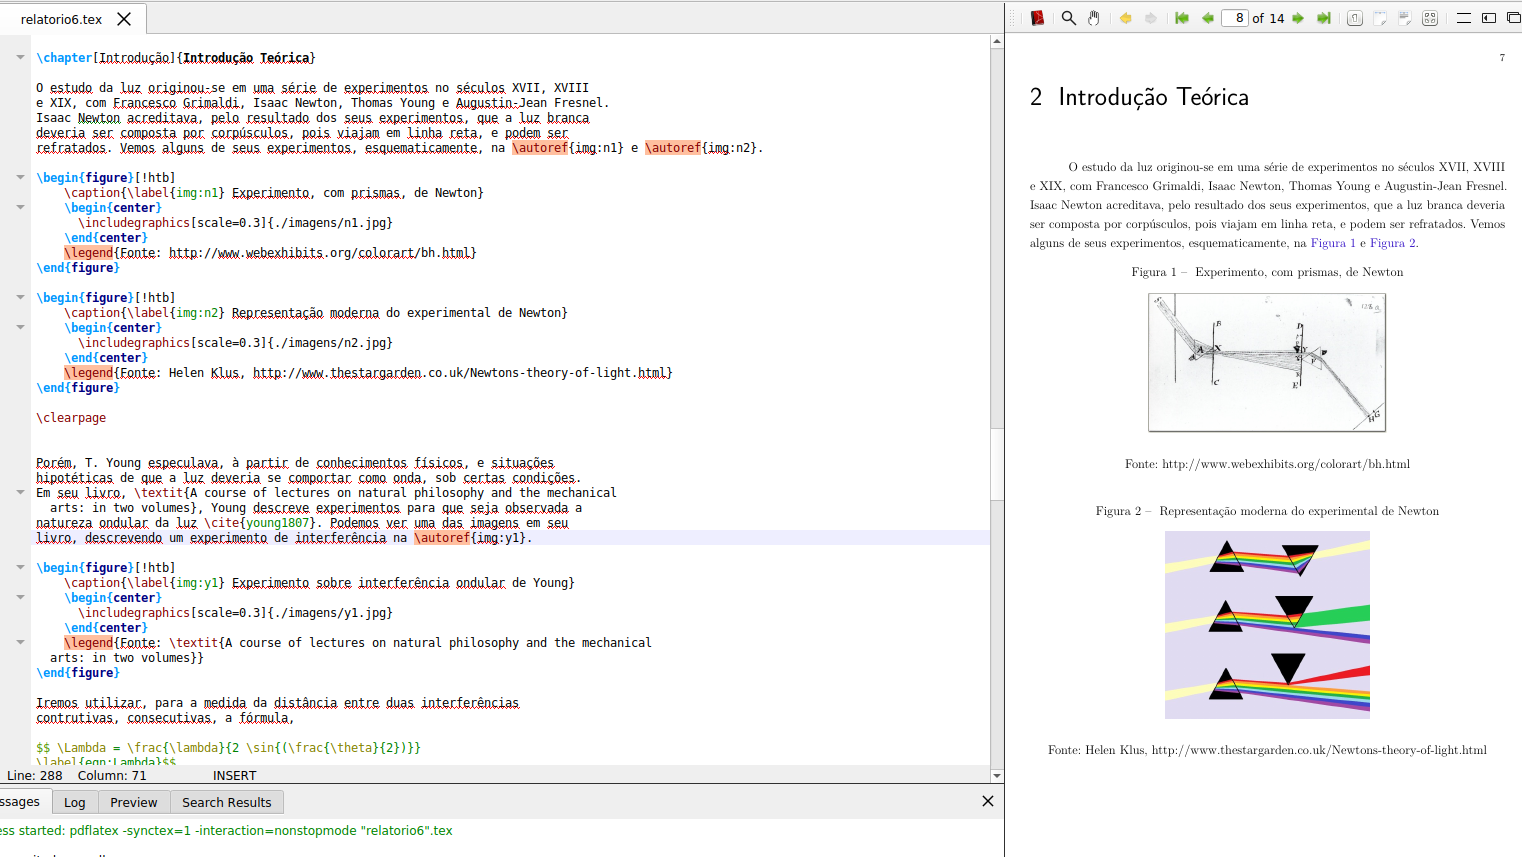
\includegraphics[scale=0.20] {../Imagens/ST3.png}
  \end{center}


\end{frame}





\begin{frame}

  \section{Exercícios}
  \frametitle{Em casa, faça os exercícios do capítulo 1}

  Os exercícios consistem em manipular parâmetros do template do
  relatório. Alguns deles são, por exemplo, a fonte, e tamanho.

  \begin{center}
    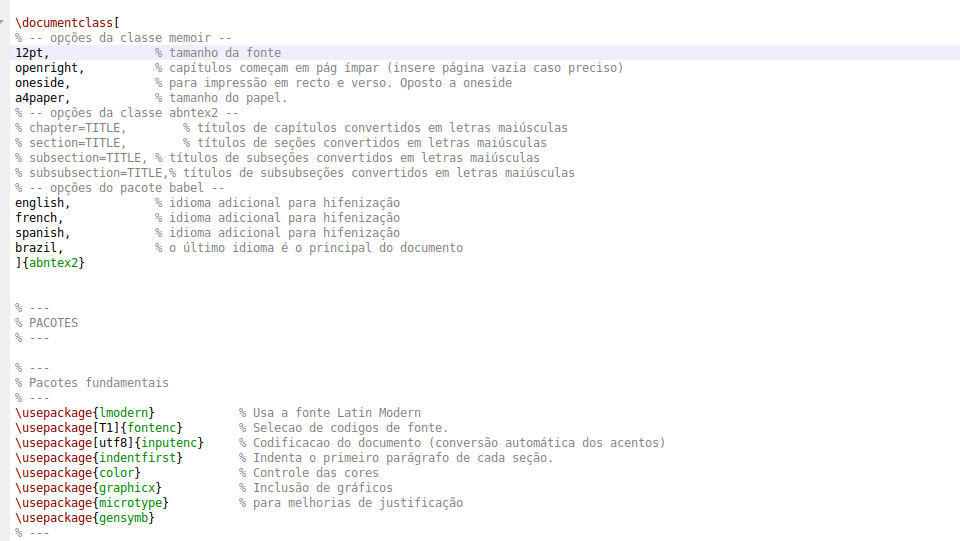
\includegraphics[scale=0.30] {../Imagens/ST4.png}
  \end{center}

  \end{frame}

  \begin{frame}

  \frametitle{Em casa, faça os exercícios do capítulo 1}

  Espaçamento de linha e parágrafo.

   \begin{center}
    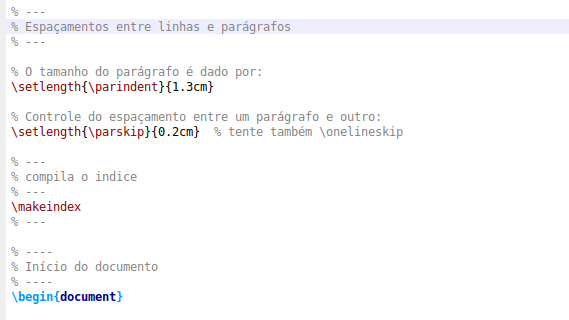
\includegraphics[scale=0.40] {../Imagens/ST5.png}
  \end{center}


\end{frame}


\end{document}

%%% Local Variables:
%%% mode: latex
%%% TeX-master: t
%%% End:
